\setcounter{page}{1}
\thispagestyle{empty}
\noindent {\fontsize{24pt}{22pt}\selectfont \booktitle\enskip--\enskip\booksubtitle} \\
{\large \bookauthor}

\bigskip

\noindent {\fontsize{16pt}{20pt}\selectfont\textcolor{titletextcolour}{\textbf{Version\,\version \enskip---\enskip Revision\,\revision}}} \\

\setlength{\parskip}{0pt}
\noindent \textbf{Original text:} Originally written by David Guichard of Whitman College, the single variable material is a modification and expansion of notes written and generously released by Neal Koblitz  of the University of Washington. That version also contains some content, exercises, and examples from \textit{Elementary Calculus: An Approach Using Infinitesimals}, written by H. Jerome Keisler of the University of Wisconsin under a Creative Commons license. Albert Schueller, Barry Balof, and Mike Wills all of Whitman College, have also contributed content.

\medskip

\noindent \textbf{Edits 2012-2014:} The majority of the text was modified and expanded by Michael Cavers of the University of Calgary.

\medskip

\noindent \textbf{Edits 2014:} Mark Blenkinsop of Carleton University further augmented and edited the content; in particular, the addition of a section on Linear and Higher Order Approximations.

\medskip

\noindent \textbf{Edits 2015:} The text has been additionally augmented and edited by Joseph Ling of the University of Calgary; specifically, new exercises, proofs for theorems, revised arrangement of topics in the chapter on Applications of Derivatives, as well as additional explanation of content and examples in the section on Continuity.

\medskip

\noindent \textbf{Edits 2016:} Much of the first two thirds modified and expanded by Tim Alderson of the University of New Brunswick Saint John. Added new problems and answers. A significant amount of material %including, but not limited to (Antiderivatives) and some material on hyperbolic functions, inverse functions, sigma notation, substitution  
was included from Apex Calculus Version 3.0, written by G. Hartman. T. Siemers and D. Chalishajar of the Virginia Military Instititue and B. Heinold of Mount Saint Mary's University also contributed to APEX Calculus. This material is released under Creative Commons license CC BY-NC (\url{https://creativecommons.org/licenses/by-nc/4.0/} ). See \url{http://www.apexcalculus.com/} for more information and original version.\\
Other material %on Riemann Sums, Definite integral, FTC, substitution has been 
was adapted from Active Calculus, by Matt Boelkins, and from the FreeCalc Project.   

\noindent \textbf{Edits 2017:}
\begin{itemize} 
   \item Lyryx: Front matter has been updated including cover page, copyright, and revision pages. 
   \item Lyryx: Examples \ref{exa:anglebetweencurves}, \ref{exa:findgrad}, \ref{exa:greenseg}, \ref{exa:conservative}, \ref{exa:lengthhelix}, \ref{exa:surfacearea}  and Exercises \ref{exfix1}, \ref{exfix2}, \ref{exfix3} have been rewritten. Several exercises from Vector Calculus have been removed.  
   \item Lyryx: Order and name of topics in Chapter \ref{chap:VectorFunctions} and Chapter \ref{chap:VectorCalculus} have been revised. 
   \item D. Guichard: New content developed for the Three Dimensions, Vector Functions, and Vector Calculus chapters.  
   \item Lyryx: Exercise numbering has been updated to restart with each section.  %\item G. Hartman: New content on Riemann Sums is included, Section %\ref{sec:riemann}. This section was adapted by Lyryx from the section of the same name in APEX Calculus, Version 3.0, written by G. Hartman. T. Siemers and D. Chalishajar of the Virginia Military Instititue and B. Heinold of Mount Saint Mary's University also contributed to APEX Calculus. This material is released under Creative Commons license CC BY-NC (\url{https://creativecommons.org/licenses/by-nc/4.0/} ). See \url{http://www.apexcalculus.com/} for more information and original version.
 \end{itemize} 

\noindent \textbf{Edits 2018:} Much of first two chapters modified and expanded by Hope Alderson of the University of New Brunswick Saint John. Added new problems and answers. A significant amount of material %including, but not limited to (Antiderivatives) and some material on hyperbolic functions, inverse functions, sigma notation, substitution  
was included from Precalculus, Version 3.0, written by Carl Stitz (Lakeland Community COllege), and Jeff Zeager (Lorain County Community College). This material is released under Creative Commons license CC BY-NC (\url{https://creativecommons.org/licenses/by-nc/4.0/} ). See \url{http://www.apexcalculus.com/} for more information and original version.\\ 
\bigskip

\noindent All new content (text and images) is released under the same license as noted below.

\vspace{5em}

\noindent Tim Alderson

\noindent University of New Brunswick Saint John

\vfill


\noindent {\fontsize{16pt}{20pt}\selectfont\textcolor{titletextcolour}{\textbf{Copyright}}} \\

\noindent 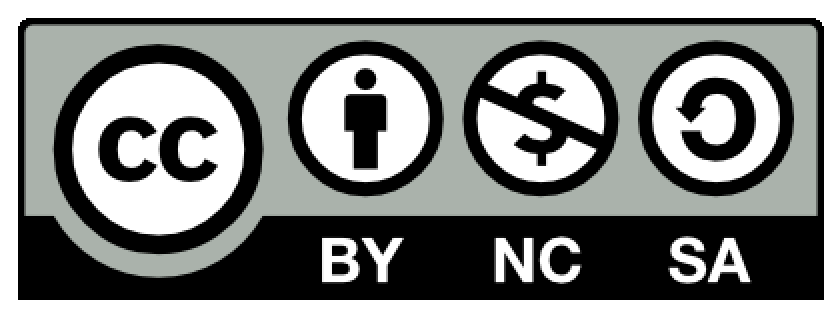
\includegraphics[width=3cm]{images/cc-by-nc-sa.eps}

\medskip

\noindent \textbf{Creative Commons License (CC BY-NC-SA)}: This text, including the art and illustrations, are available under the Creative Commons license (CC BY-NC-SA), allowing anyone to reuse, revise, remix and redistribute the text.  

\medskip

\noindent To view a copy of this license,
visit \href{http://creativecommons.org/licenses/by-nc-sa/3.0/}{http://creativecommons.org/licenses/by-nc-sa/3.0/}  

\setlength{\parskip}{\baselineskip}